\documentclass[tikz,border=2mm]{standalone}
\usepackage{ctex}
\tikzset{global scale/.style={
    	scale=#1,
    	every node/.append style={scale=#1}
  	}
}
\begin{document}
	%开始绘图
	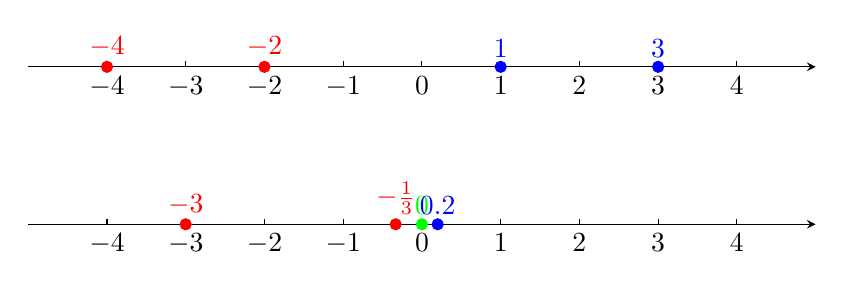
\begin{tikzpicture}[global scale = 1]
  		\draw [black, ->, >=stealth] (-5,0) -- (5,0); 
		\foreach \x in {-4, ..., 4}
			\draw (\x cm,2pt) -- (\x cm,0pt) node[anchor=north] {$\x$};
		% 1, -2, 3, -4
		\draw [blue, fill=blue] (1, 0) circle(2pt) node [above] {$1$}; 
		\draw [red, fill=red] (-2, 0) circle(2pt) node [above] {$-2$}; 	
		\draw [blue, fill=blue] (3, 0) circle(2pt) node [above] {$3$}; 
		\draw [red, fill=red] (-4, 0) circle(2pt) node [above] {$-4$}; 			
		% -1/3, 0, -3, 0.2
		\draw [black, ->, >=stealth] (-5,-2) -- (5,-2); 
		\foreach \x in {-4, ..., 4}
			\draw (\x cm,-2cm+2pt) -- (\x cm,-2cm+0pt) node[anchor=north] {$\x$};
		\draw [red, fill=red] (-1/3, -2) circle(2pt) node [above] {$-\frac{1}{3}$}; 
		\draw [green, fill=green] (0, -2) circle(2pt) node [above] {$0$}; 					 		
		\draw [red, fill=red] (-3, -2) circle(2pt) node [above] {$-3$}; 
		\draw [blue, fill=blue] (0.2, -2) circle(2pt) node [above] {$0.2$}; 					
	\end{tikzpicture} 
	%结束绘图
\end{document}
